\documentclass{beamer}
\beamertemplatenavigationsymbolsempty
\usecolortheme{beaver}
\setbeamertemplate{blocks}[rounded=true, shadow=true]
\setbeamertemplate{footline}[page number]
%
\usepackage[utf8]{inputenc}
\usepackage[english,russian]{babel}
\usepackage{amssymb,amsfonts,amsmath,mathtext}
\usepackage[]{algorithmic}
\usepackage{subfig}
\usepackage[all]{xy} % xy package for diagrams
\usepackage{array}
\usepackage{tikz}
\usepackage{multicol}% many columns in slide
\usepackage{hyperref}% urls
\usepackage{hhline}%tables
% Your figures are here:
% \graphicspath{ {fig/} {../fig/} }

%----------------------------------------------------------------------------------------------------------
% \title[\hbox to 56mm{}]{}
% \author[]{}
% \institute{Московский физико-технический институт}
% \date{\footnotesize
% \par\smallskip\emph{Курс:} 
% \par\smallskip\emph{Эксперт:} 
% \par\smallskip\emph{Консультант:}
% \par\bigskip\small 2021}
%----------------------------------------------------------------------------------------------------------
\begin{document}
%----------------------------------------------------------------------------------------------------------
% \begin{frame}
% \thispagestyle{empty}
% \maketitle
% \end{frame}
%-----------------------------------------------------------------------------------------------------

%-----------------------------------------------------------------------------------------------------
\begin{frame}{Петли в рекомендательных системах}

\begin{columns}[c]
\column{0.5\textwidth}
Отклик $c_t^i$ для рекомендации $\mathbf{a_t}$:
\begin{gather*}
    c_t^i \sim \text{Bern} \left(\sigma\left(\mu_t^i (a_t^i) + \mathbin{\color{red} q_t^i } \right) \right). 
\end{gather*}
Интерес $\mu_t^i$:
\begin{gather*}
    \mu_{t+1} - \mu_{t} = \delta_t c_t - \delta_t (1 - c_t),\\ 
\end{gather*}

Определение петель: 
\begin{gather*}
  \color{red} \lim_{t \to \infty} \|\mu_t - \mu_0 \|_2 = \infty.
\end{gather*}
\column{0.6\textwidth}



% \begin{tikzpicture}[
%   node distance={13mm}, thick, 
%   roundnode/.style={circle, draw=blue!60, fill=blue!5, very thick, minimum size=4mm},
%   squarednode/.style={rectangle, draw=red!60, fill=red!5, very thick, minimum size=4mm},
% ] 
% \node[roundnode] (1) {$a^1$}; 
% \node[roundnode] (2) [right of=1] {$a^2$};
% \node[roundnode] (3) [right of=2] {$a^3$};
% \node[squarednode] (5) [below of=1]{$\mu^1$}; 
% \node[squarednode] (6) [below of=2] {$\mu^2$};
% \node[squarednode] (7) [below of=3] {$\mu^3$};
% \node[draw] (4) [below of=6] {$User$};

% \draw[-] (4) -- (5);
% \draw[-] (4) -- (6);
% \draw[-] (4) -- (7);

% \draw[blue,->] (5) to [out=150, in=-150, looseness=1.] node[left]{$c^1 = 1$} (1);
% \draw[blue,->] (6) to [out=150, in=-150, looseness=1.]  (2);
% \draw[blue,dotted] (7)  to [out=150, in=-150, looseness=1.] node[right]{$c^3 = 0$} (3);

% \draw[red,->] (1) to [out=-30, in=30, looseness=1.] node[left]{$+\delta^1$}(5);
% \draw[red,->] (2) to  [out=-30, in=30, looseness=1.] (6);
% \draw[red,->] (3) to  [out=-30, in=30, looseness=1.]node[right]{$-\delta^3$}(7);
% \end{tikzpicture} 
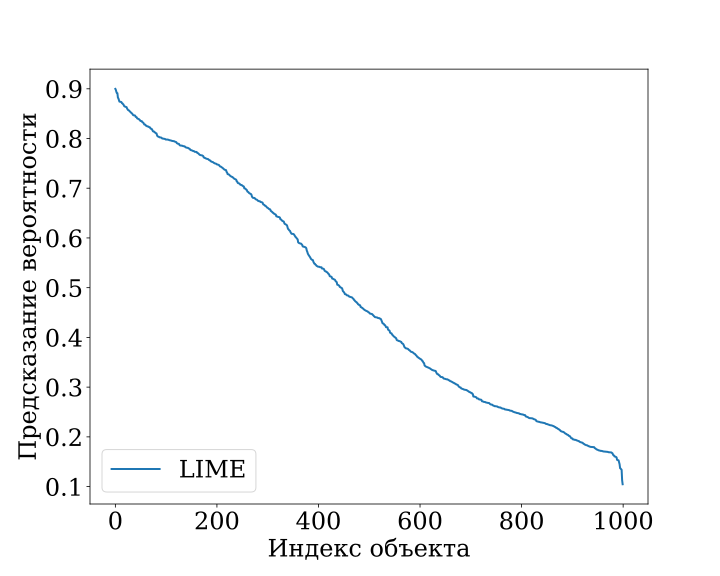
\includegraphics[width=7cm]{../figures/lime_proba.svg}
\end{columns}
\end{frame}


\end{document} 